\chapter{The Web Browser User Interface}
\label{shui}
\index{shui}
The \zwshui is considered the main control interface of \zway. 

A screenshot overview is shown in Figure \ref{sh2} marking the essential parts of 
the interface.  It looks similar on different devices 
such as a desktop PC, smartphone, and tablet (both native app and browser), but will 
adapt to the screen size. 

The \zwshui follows some very clear logic thats was developed by Prof. Christian 
Paetz and presented the first time on the Smart Home Summit 2014 in Munich/Germany.
Annex \ref{slides} shows the short slide deck of this initial presentation.

The following basic rules apply:

\index{Elements}
\index{Elements Configuration}
\index{Events}
\index{Apps}

\begin{enumerate}

\item \textbf{Elements}: Every function of any device is shown as one single (No. 7). (In case a 
physical device has multiple functions, like switching and metering, it will be offered 
as multiple elements). All elements are listed in the elements view (No. 3) and can be 
filtered by function 
type (switch, dimmer, sensor) or other filtering criteria.

\item \textbf{Elements Configuration}: Every element offers a configuration interface (No. 8) for changing names, removing 
it from the screens, etc. Important elements can be placed in the Dashboard (No. 1). 

\item \textbf{Event}: Every change in a sensor value or a switching status is called an 
``Event’’ and is shown  in the timeline (No. 4). Filtering allows monitoring the changes in one single function 
or device. Besides, elements can be assigned to different rooms (No. 2).


\item \textbf{Apps}: All other functions such as time-triggered actions, the use of information from the 
internet, scenes plugin of other technologies, and services are realized in apps accessible 
in the setup menu (No 6). These apps are ready-to-use scripts/templates that can add extra 
logic and functionality such as logic rules like ``IF->THEN,’’ scene definitions, timers, 
and interactions with external (non-\zwave) devices connected via USB dongle or via 
internet. Some apps are built into the system. More can be downloaded from an app store. 
To use an app, you create an instance of this app and configure its properties. If useful, 
you can create more than one instance of one single app. The apps can create none, one, or 
multiple new elements and events. You can install new apps and manage them using the menu
Configuration -> Apps.

\end{enumerate}

\begin{figure}
\begin{center}
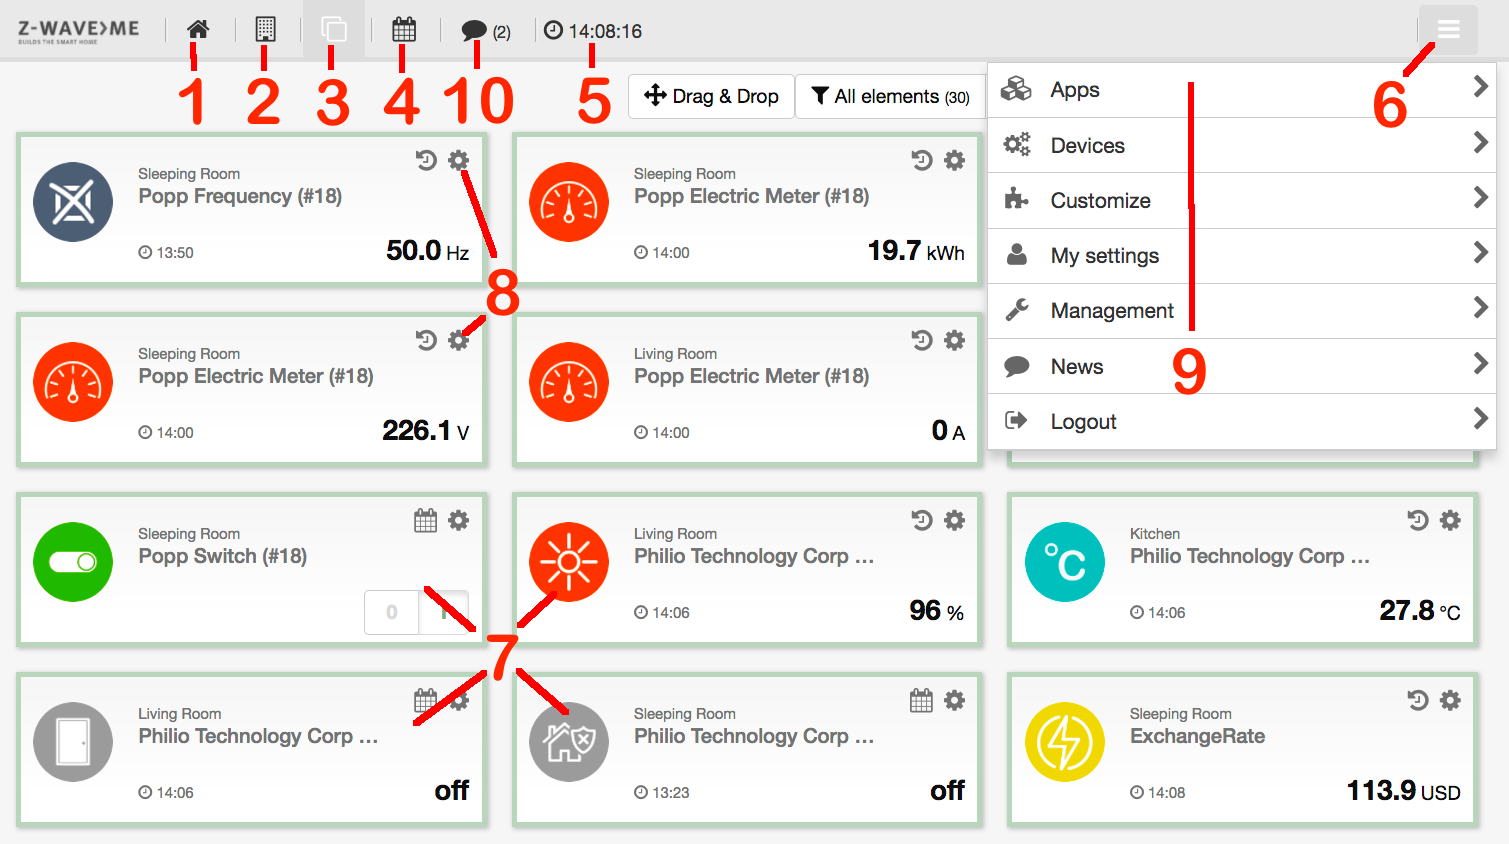
\includegraphics[width=1.0\textwidth]{pngs/cap4/shui1a.png}
\caption{\zwshui}
\label{sh2}
\end{center}
\end{figure}


\section{\zwshui Daily Usage}

 
\subsection{Standard Element View}

Figure \ref{sh2} shows the standard element view of the \zwshui. 
Elements with an icon, buttons, or variables are placed side by side. Depending on the 
screen size, they are grouped in one (mobile phone), two (pad), or three (PC screen) 
columns.

The very same display is available on the \keystroke{Dashboard} (No. 1), the \keystroke{Room View} (No. 2), 
and the \keystroke{Element view} (No. 3). The element view shows all elements (No. 7) available
while the dashboard shows elements that where manually selected for display on the 
dashboard. The clock on the topline menu (No. 5) shows the actual time in the time 
zone of the gateway (not the actual position of the browser). The elements can be filtered 
by element type or can be ordered by

\begin{itemize}
\item Time of creation (ascending or descending)
\item Given name in alphabetical order (ascending or descending)
\item Last update
\item Custom
\end{itemize}

The button \keystroke{Drag-and-Drop} turns the user interface in a reordering mode. Just drag and drop 
elements to reorder them. After the new order is saved, it is available as 'custom'. The 
same logic can be applied to all view showing elements (Element View, Dashboard, and Room 
View).

A search field allows searching for given names of the elements.

All elements can be assigned to ``tags’’: Tags are text blocks that can be arbitrarily 
chosen. Typical tags are ``Temperatures,’’ ``Energy,’’ and ``Outdoor.’’  Multiple elements 
can have the same tag and one element can have several tags. By selecting a tag, only 
elements are shown that are tagged with this name.

Tags are managed on the element configurations described below.

\begin{figure}
\begin{center}
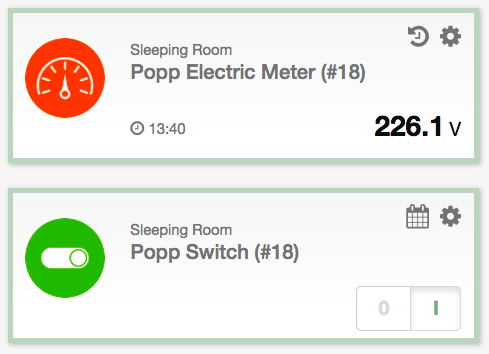
\includegraphics[width=0.4\textwidth]{pngs/cap4/sh4.png}
\caption{Elements}
\label{sh4}
\end{center}
\end{figure}

Figure \ref{sh4} shows two typical elements:
Each element has a given name. This name may refer to the function or the position. Please 
make sure to keep the name short enough so that no display problem is created. Each element 
also has one or several icons. In case the element represents an actor function, the icon 
usually refers to the switching state of the actor (on or off, up or down). Changing icons 
also indicate the status of binary sensors such as motions detectors.
Analog sensors typically only have one icon. The upper element is an actor allowing to 
be switched on and off. 

%Additionally, this element allows changing a color. Clicking on the 
%small triangle right to the word RGB will open a color picking sub-dialog. Above the 
%given name is the room name if the element is assigned to a room.

The 
\includegraphics[width=0.04\textwidth]{pngs/wheel.png} (No. 8 on Figure \ref{sh2}) on 
the right-hand side opens the element configuration dialog. The symbol left to the configuration 
wheel depends on the type of device. For devices with analog values such as rain sensors, 
temperatures, etc., the icon 
\includegraphics[width=0.04\textwidth]{pngs/24hour.png} will 
open a 24-hour history of the sensor value. Devices 
with 24-hour history also show a time stamp when the last value update was received. 
Clicking on the large icon itself will call for a value update, but please keep in mind 
that battery-operated devices will only send updated values after the next wakeup.
For event-driven devices such as actuators or binary sensors, an icon 
\includegraphics[width=0.04\textwidth]{pngs/10events.png}
will show a list 
of the last 10 events with the time stamp. One click away is then the full list of 
events, as described in Section \ref{timeline}, but filtered for this element.

\subsubsection{Element Configuration}
\label{ElementConfiguration}

Every element shown has its own configuration dialog (No. 7 on \ref{sh2}). Clicking 
on the 
\includegraphics[width=0.04\textwidth]{pngs/wheel.png} symbol on the upper right-hand 
side opens this dialog.

\begin{figure}
\begin{center}
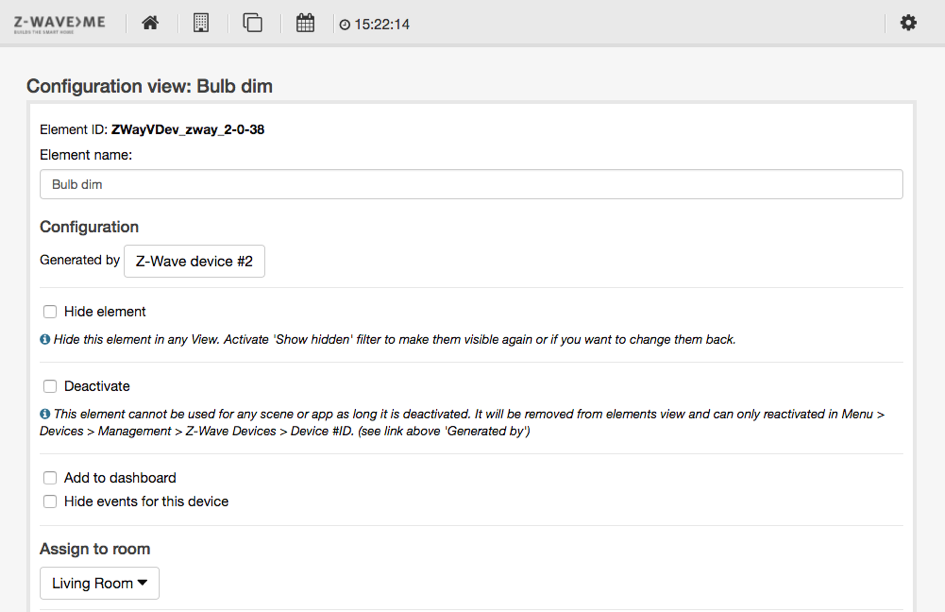
\includegraphics[width=0.9\textwidth]{pngs/cap4/sh5.png}
\caption{Elements configuration - upper part}
\label{sh5}
\end{center}
\end{figure}

Figure \ref{sh5} shows the upper part of the element configuration dialog.

The element ID is an internal reference and for advanced scripting only. The element name 
is the given name of the element. \zway tries to automatically find a reasonable name, but 
the user should change this name according to the specific setup of the home.

\begin{itemize}
\item Generated By: This refers to the physical device of the \zway application that 
generated this element. In the example above, this device is the physical \zwave device 
with Node ID 2. Clicking on the button with the name of the element-creator leads to the 
configuration dialog of the physical device, i.e. the \zway application.

\item Hide element: As explained in the dialog, this checkbox will hide the element. However, 
this setting can be reversed by showing hidden devices. This setting is for cosmetic view only.

\item Deactivate: This checkbox allows removing the element. It will not only disappear 
from the element view but also from any dropdown list to setup device relationships, etc. 
For information on how to re-activate such an element, refer to the user settings dialog 
description in Section \ref{mysettings}.

\item Add to Dashboard: This places the element on the dashboard.

\item Hide events from this device: This keeps the device in the element view or Dashboard, but 
no events of this device will be shown in the event timeline.

\item Assign to room: This allows assigning this element to a certain room or changing 
this assignment.

\end{itemize}

\begin{figure}
\begin{center}
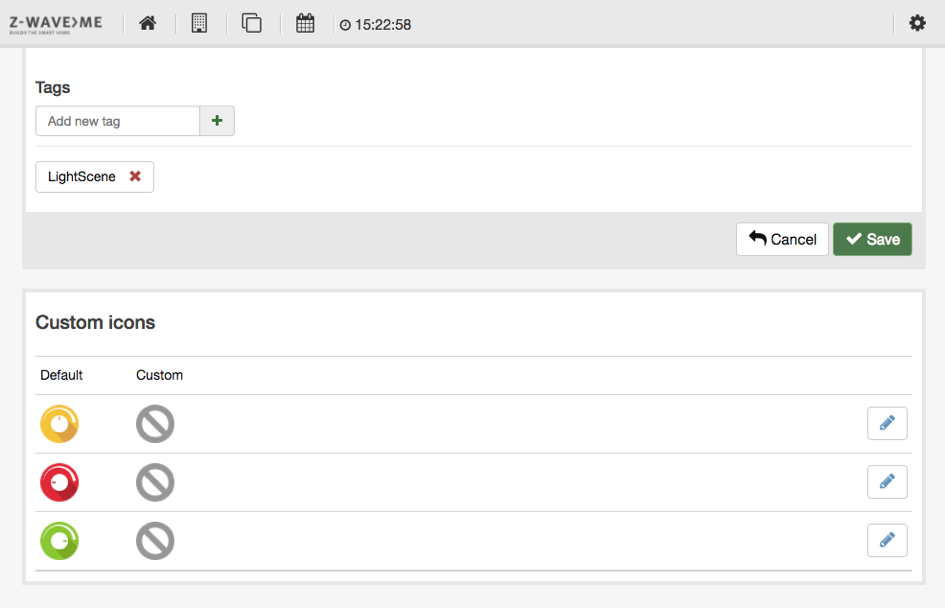
\includegraphics[width=0.9\textwidth]{pngs/cap4/sh6.png}
\caption{Elements configuration  - lower part}
\label{sh6}
\end{center}
\end{figure}

Figure \ref{sh6} shows the lower part of the element configuration dialog. The tag option 
allows setting and removing tags. When a tag name is inserted into the text field, it 
autocompletes known tag names.

The custom icon sub-dialog allows changing the icons of the element. Each element has one, 
two, or three icons depending on the status indicated. Each of the icons can be replaced 
by an own individual icon. Just click on the pencil button to change the icon. To 
download more icons, refer to the customization section in the configuration menu.

\subsubsection{Room View}
\index{Rooms}

The \zwshui allows managing different rooms and assigning elements to 
rooms. Each element can be placed in one room only.

Clicking on the room symbol on the top menu opens the room view with a list of rooms, 
as shown in Figure \ref{roomover}.

\begin{figure}
\begin{center}
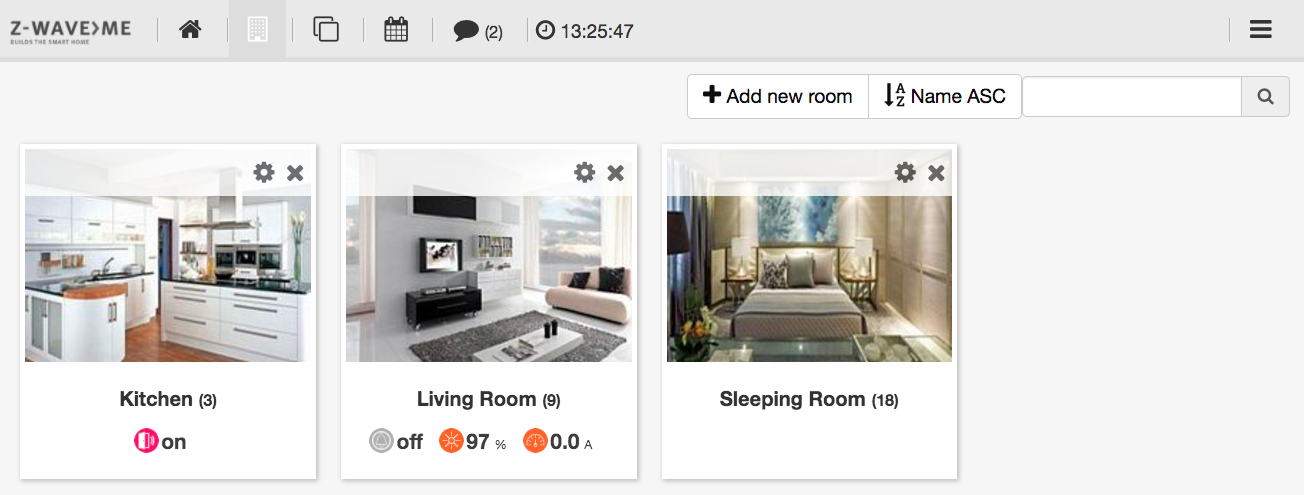
\includegraphics[width=0.9\textwidth]{pngs/cap4/roomover.png}
\caption{Room overview}
\label{roomover}
\end{center}
\end{figure}

Each room has its own element with a background image that can be configured. It is 
possible to add new rooms using the button labeled \keystroke{Add room}.
The room is named and the number of elements in this room is shown. Per room there 
are up to three sensors that can be selected as ``quick-view sensors’’. They are shown 
right below the name and in the top menu in the individual room view.

Clicking on the room element leads to the room view, as shown in Figure \ref{roomview}.

\begin{figure}
\begin{center}
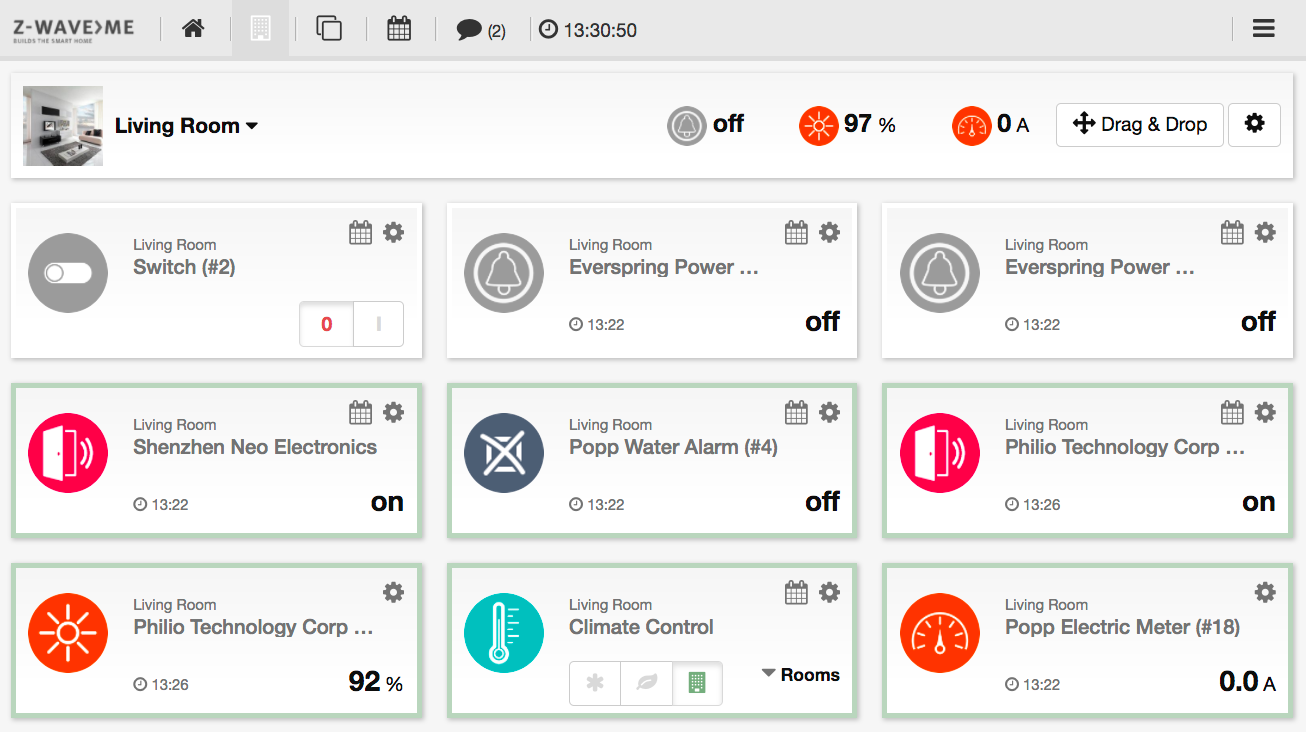
\includegraphics[width=0.9\textwidth]{pngs/cap4/roomview.png}
\caption{Room View}
\label{roomview}
\end{center}
\end{figure}

The room view lists all the elements in the room. As in the element view, they can be 
re-arranged using the drag-and-drop feature.

The top line shows up to three quick sensors and allows quick change of the room using 
the dropdown list. If your browser supports gestures, you can change the rooms by 
swiping left or right.

Clicking on the 
\includegraphics[width=0.04\textwidth]{pngs/wheel.png} symbol of the 
room element or inside the room view in the top line opens the room configuration 
dialog, as shown in Figure \ref{sh7}.

\begin{figure}
\begin{center}
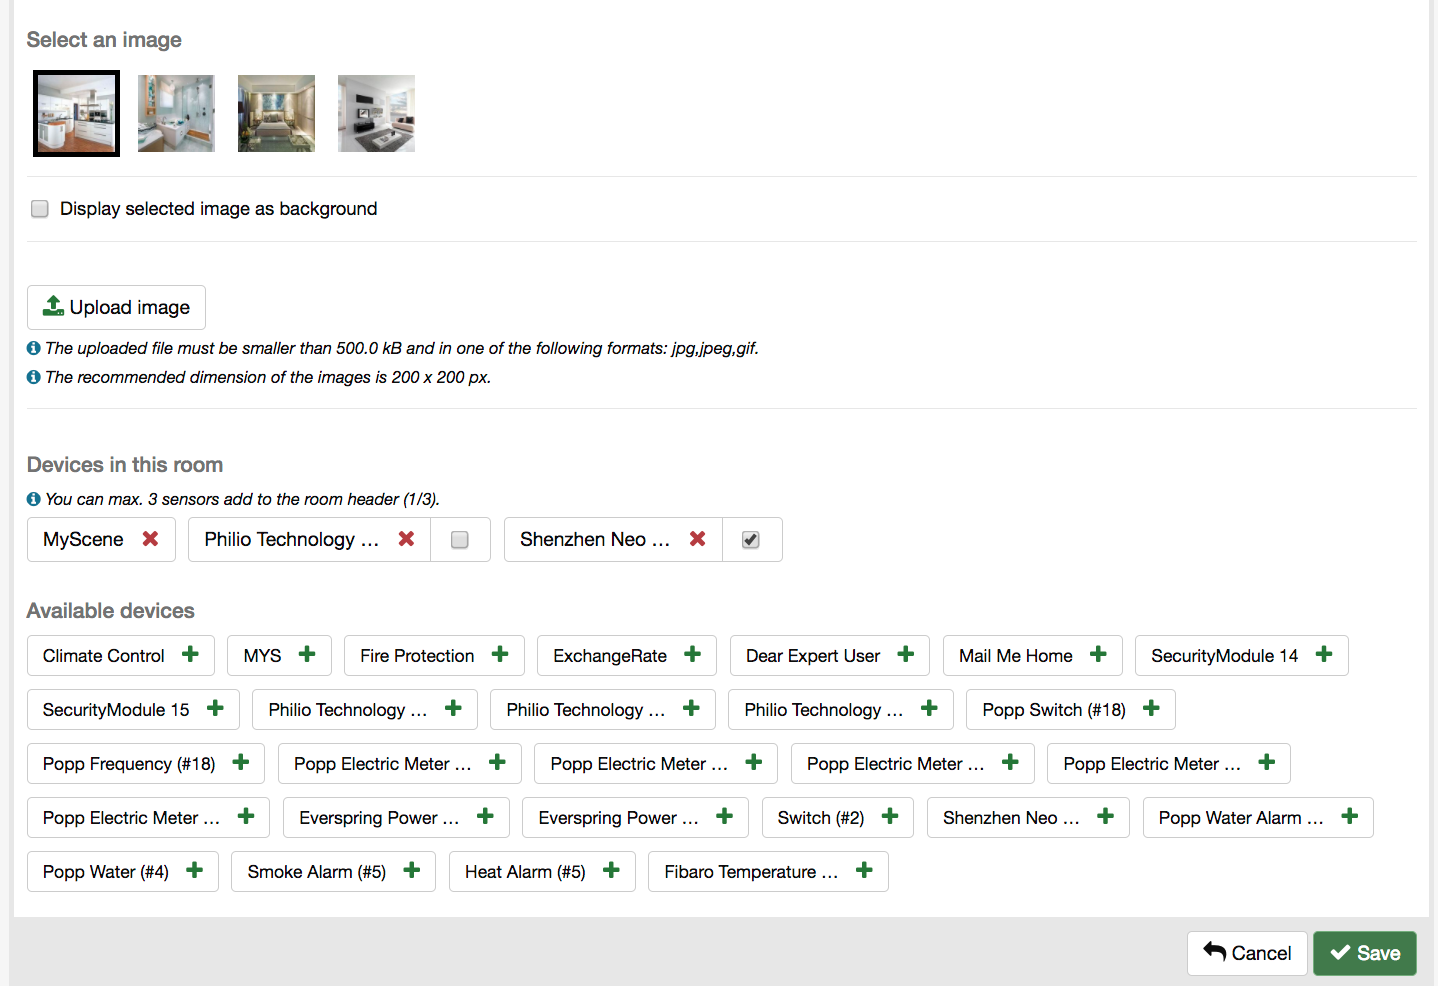
\includegraphics[width=0.9\textwidth]{pngs/cap4/sh7.png}
\caption{Room configuration dialog}
\label{sh7}
\end{center}
\end{figure}

Each room can have an individual name. Besides some pre-installed images, it is possible 
to upload images for the room. A checkbox defines the room image that is used as a 
background image in the room view.

The dialog allows assigning elements to this room which were not assigned to any room 
yet. Just click on the element name in the list of \keystroke{Available devices}.

The little checkbox on the right-hand side allows selecting up to three sensors as 
``quick-view sensors’’.

\subsubsection{Event Timeline}
\label{timeline}

The event timeline is the forth menu item in the top menu.

\begin{figure}
\begin{center}
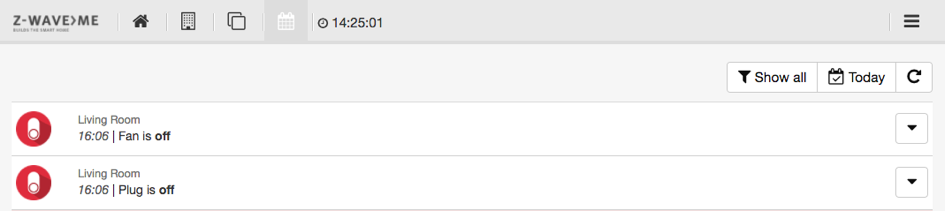
\includegraphics[width=0.9\textwidth]{pngs/cap4/sh8.png}
\caption{Timeline}
\label{sh8}
\end{center}
\end{figure}

The timeline dialog offers a chronological view of the events in the Smart Home. The events 
are:

\begin{itemize}
\item Change of status of actuators such as dimmers, blind controls, or switches
\item Tripping of binary sensors (motion, door, etc.)
\item Change of measured value of sensors
\item Network status changes (device lost, device back, etc.)
\end{itemize}

The standard view of the timeline, as shown in Figure \ref{sh8}, lists all events with the 
icon of the element, room info, time stamp, name of the element, and status info. Every 
line item has a context menu on the right-hand side. This menu allows

\begin{itemize}
\item showing events of this source element only,
\item showing events of this event type only,
\item showing events that have the same event type,
\item directly moving to the element configuration page of this element,
\item hiding all events from this source.
\end{itemize}

\subsection{News feed}
\index{News Feed}

 Each \zway controller is connected to an RSS feed. This feed contains news and alerts 
 about the platform. Whenever there is a new feed entry, the top menu bar will indicate 
 this with a sign, as shown with Marker 1 in Figure \ref{news1}. Clicking on this opens 
 the full list of news. This full list can also be accessed using the 'News' menu 
 item in the configuration section, as described in Section \ref{news}.

\begin{figure}
\begin{center}
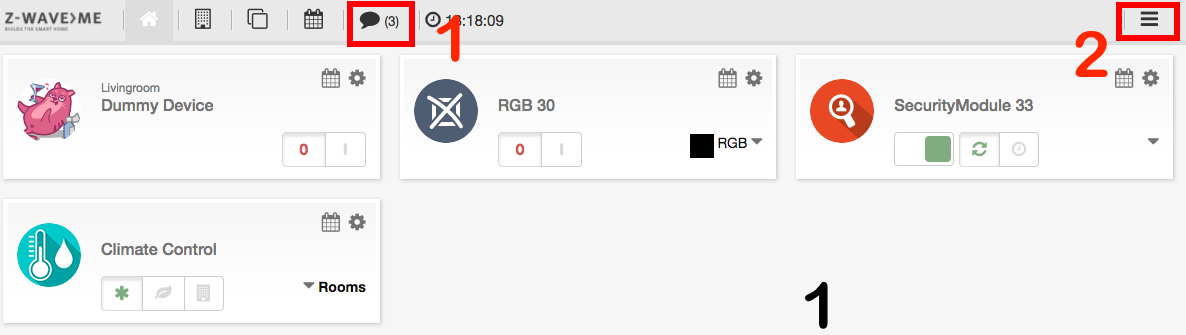
\includegraphics[width=0.9\textwidth]{pngs/cap4/news1.png}
\caption{News Indicator}
\label{news1}
\end{center}
\end{figure}

\section{The Configuration Menu}

Clicking on the menu item (marked as No. 2 in Figure \ref{news1}) on the right-hand side 
opens the configuration menu. The configuration offers various functions to enhance and 
configure the smart home system as such and the user interface. Figure \ref{sh9} shows the configuration menu of \zway.

\begin{figure}
\begin{center}
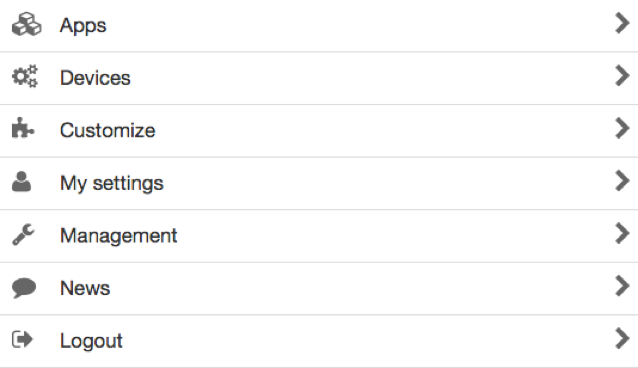
\includegraphics[width=0.9\textwidth]{pngs/cap4/sh9.png}
\caption{Configuration menu}
\label{sh9}
\end{center}
\end{figure}



\subsection{Apps}
\label{appssetup}
\index{Apps}

This menu option allows managing the home automation applications and interfaces of 
Internet or IP-based services or devices.

\zway apps are like software applications that use the infrastructure of the \zwave 
network to provide application solutions and dependencies. These software applications also 
extend the capabilities of the network and implement automation functions.

\begin{figure}
\begin{center}
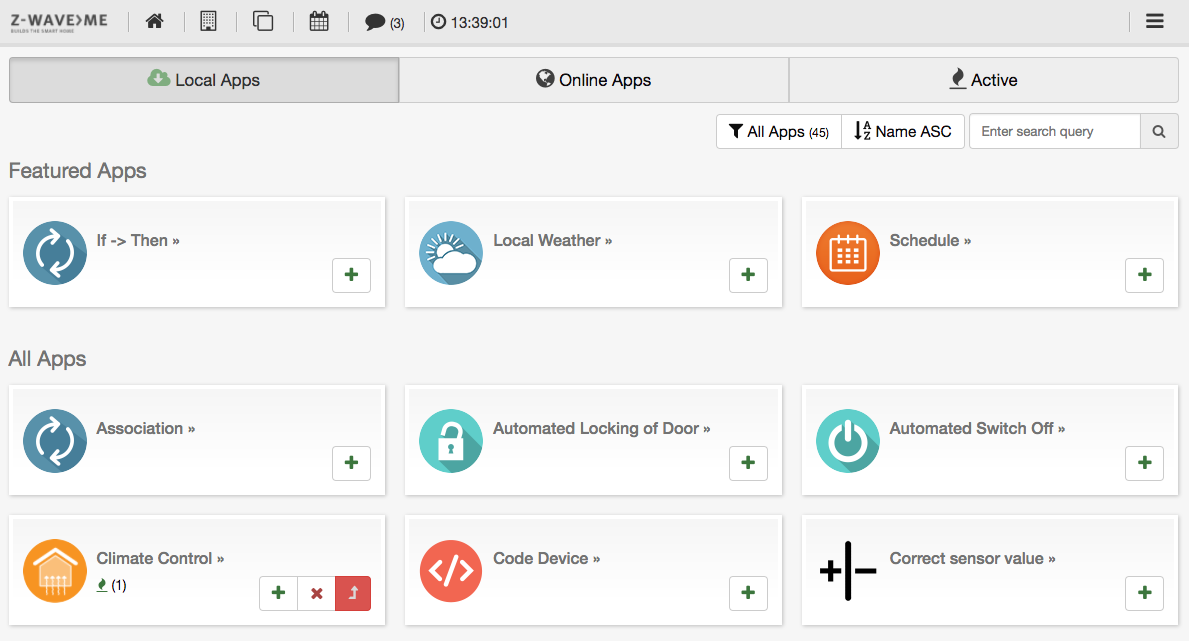
\includegraphics[width=0.9\textwidth]{pngs/cap4/app2.png}
\caption{Local Apps}
\label{app2}
\end{center}
\end{figure}

Like any other application software such as those for PCs, some \zway apps are preinstalled 
on the device, and others can be downloaded and installed by the user. Like application 
software, some software solutions can only run once while others can be started multiple times.


\begin{figure}
\begin{center}
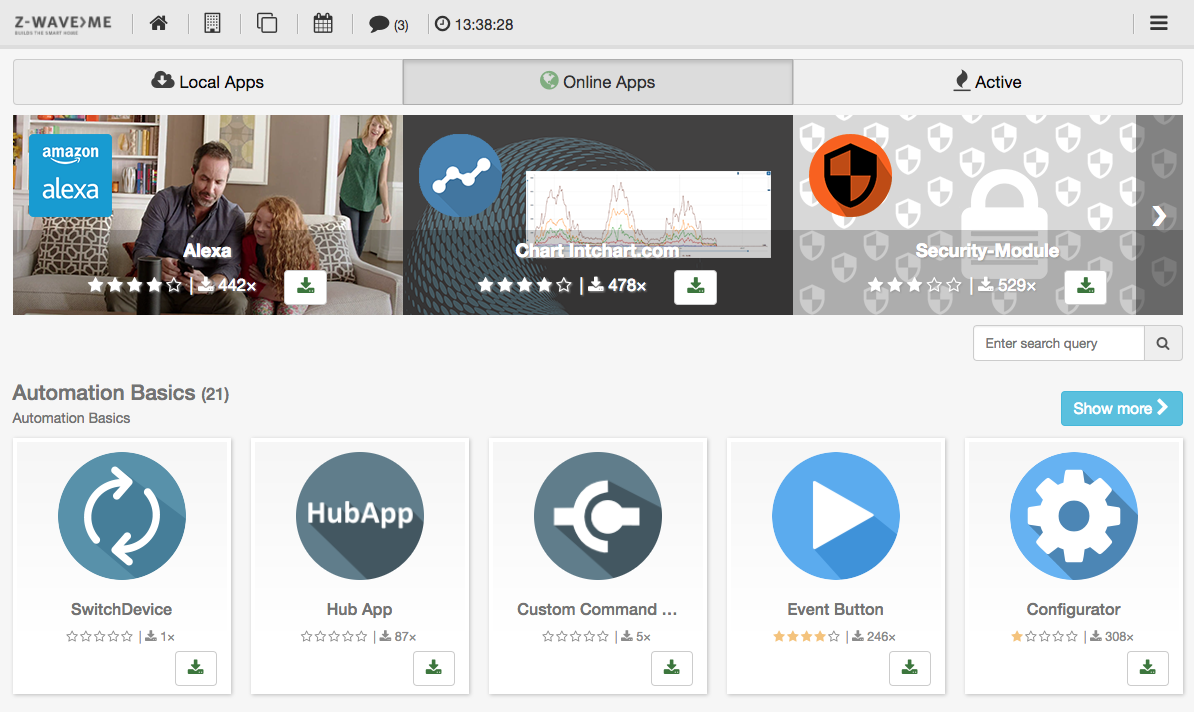
\includegraphics[width=0.9\textwidth]{pngs/cap4/app1.png}
\caption{Online Apps}
\label{app1}
\end{center}
\end{figure}

The app menu has three parts:

\begin{itemize}
\item List of apps locally available for use.
\item List of apps available on the central server and ready for download.
\item List of apps that are active and running.
\end{itemize}

The list of local apps, as displayed in Figure \ref{app2}, shows a small subset of apps that 
are already on the local devices. The top part shows some of the apps that are most 
frequently used (featured apps). A filter allows filtering for certain app types; 
ordering and direct search in the search box also help to find the right app. If 
there are active instances of the app (software running x times with different
 parameters), this is indicated right below the name of the app.

\begin{figure}
\begin{center}
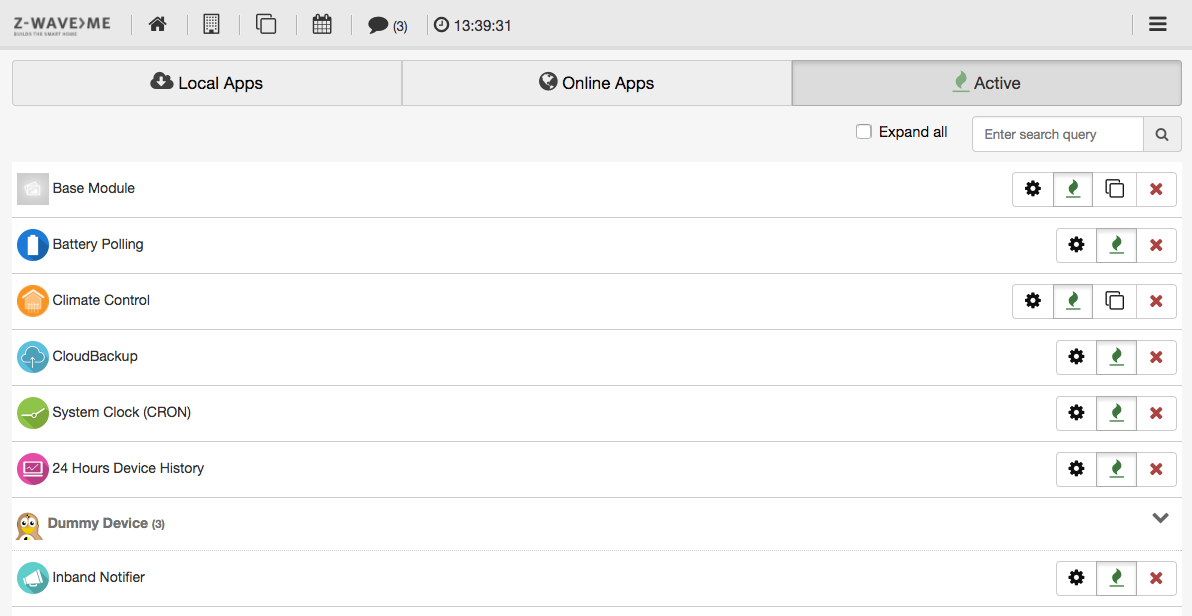
\includegraphics[width=0.9\textwidth]{pngs/cap4/app3.png}
\caption{App Setup}
\label{app3}
\end{center}
\end{figure}

Clicking on the name will open a dialog with further information about the app. Clicking 
on the \keystroke{+} button will lead right to the configuration page of the app.

The online app list, as shown in Figure \ref{app1}, offers the same functions. However, 
apps need to be downloaded first before they can be configured and started. Clicking on 
the download button will copy the app to the local repository and start the configuration 
dialog, as shown in Figure \ref{app3}.

Each app has its own name that can be changed. Depending on the function of the app, 
there are several different setup parameters.

\textbf{Please note again that some apps can be started multiple times while other 
apps are ``singletons.’’ They must only run once on the system. Once they run, they 
will disappear from the repository since they cannot be started again. Configuration
 of such a singleton is still possible using the menu of running apps. If such an app 
 stops, the app entry will reappear in the local repository.}

\begin{figure}
\begin{center}
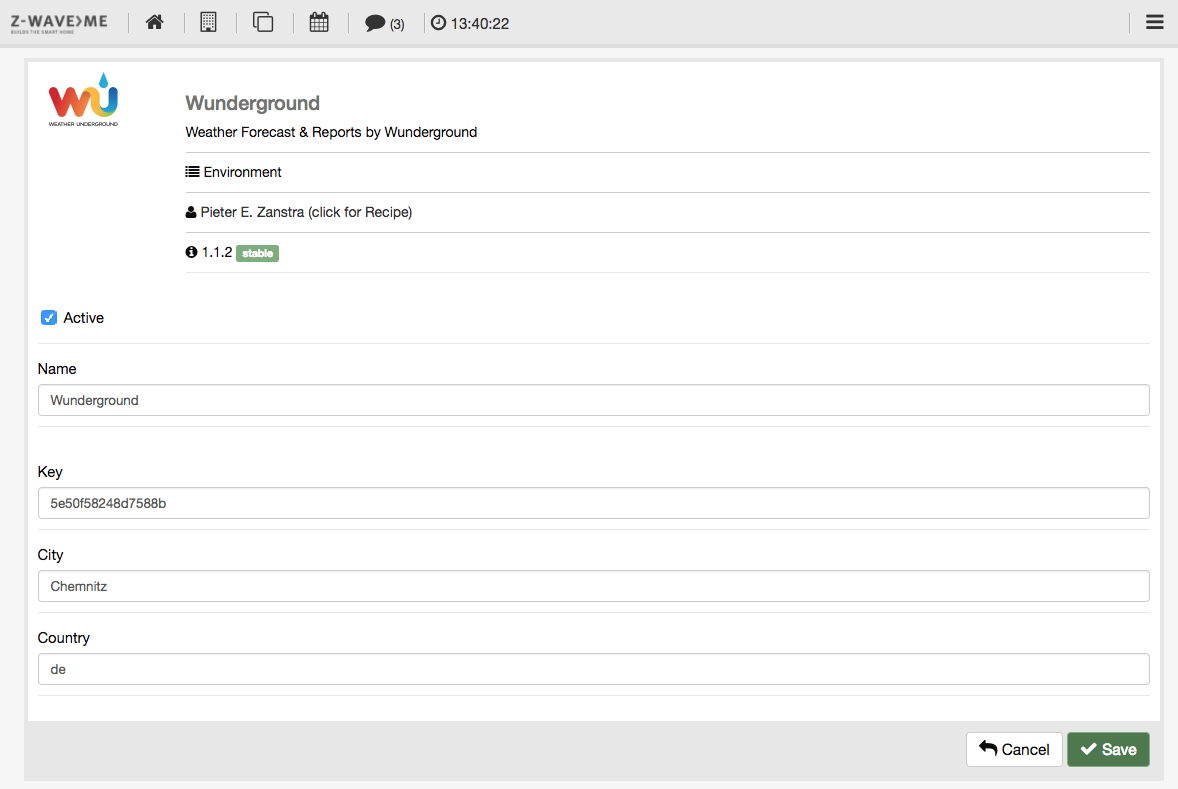
\includegraphics[width=0.9\textwidth]{pngs/cap4/app4.png}
\caption{Active App Management}
\label{app4}
\end{center}
\end{figure}

The tab for active app management is shown in Figure \ref{app4}. It lists all active 
apps by app type. If there are more than one app of the same type (e.g. \app{IF->THEN} is 
usually needed multiple times), the view is collapsed for this type of application but 
can be expanded. It is possible to expand all sections of multiple app types using the 
checkbox on the top. It is also possible to search for certain app names.

Every app line has a submenu with the following functions:

\begin{itemize}
\item 
\includegraphics[width=0.04\textwidth]{pngs/redcross.png}: Stop this app
\item 
\includegraphics[width=0.04\textwidth]{pngs/double.png}: Allows cloning an app. This will open a dialog for a new instance of the 
same app with the same settings. After saving these settings, the new app becomes active 
and is shown in the list too.
\item 
\includegraphics[width=0.04\textwidth]{pngs/greenflame.png}: Stop the App. It remains configured but is inactive. Once inactive, 
the green flame changes into a red ON button to restart the app.
\item 
\includegraphics[width=0.04\textwidth]{pngs/wheel.png}: Opens the configuration dialog. This is the very dialog to be completed 
during the initial start of the app.
\end{itemize}

Please refer to Chapter \ref{apps} for more information on different apps.

\subsection{Devices}
\index{Devices}

\begin{figure}
\begin{center}
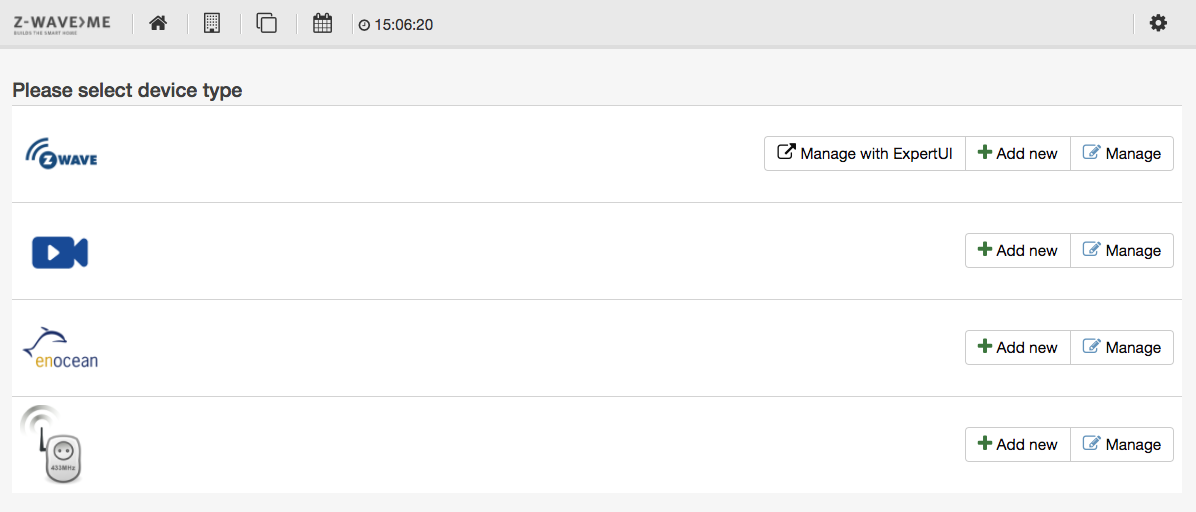
\includegraphics[width=0.9\textwidth]{pngs/cap4/433_5.png}
\caption{Device Management Overview}
\label{device0}
\end{center}
\end{figure}


The device menu allows managing physical devices. By default, it offers two physical 
device types: ``\zwave devices’’ and ``IP cameras.’’ However, if other wireless communication 
technologies are activated, they will be shown as well. Please refer to 
Chapter \ref{extensions} for more information on how to integrate further 
wireless technologies.   This section will also explain how to include/exclude and manage 
these devices and IP cameras.

Figure \ref{device0} shows the device list including EnOcean and 433 MHz devices.

Therefore, let us focus here on managing \zwave devices. Besides the standard buttons 
to add and manage devices of the specific communication technology, \zwave offers one
 more button to link to a specific second \zwave user interface for installers and professionals.
Please refer to Chapter \ref{expertuserinterface} for a detailed description of this very 
technical, the so-called \zweui. Please note that all day-to-day management functions 
can be done without involving this very specific and technical interface.

\subsubsection{Inclusion}
\label{inclusion}
\index{Inclusion}
\index{Exclusion}

\begin{figure}
\begin{center}
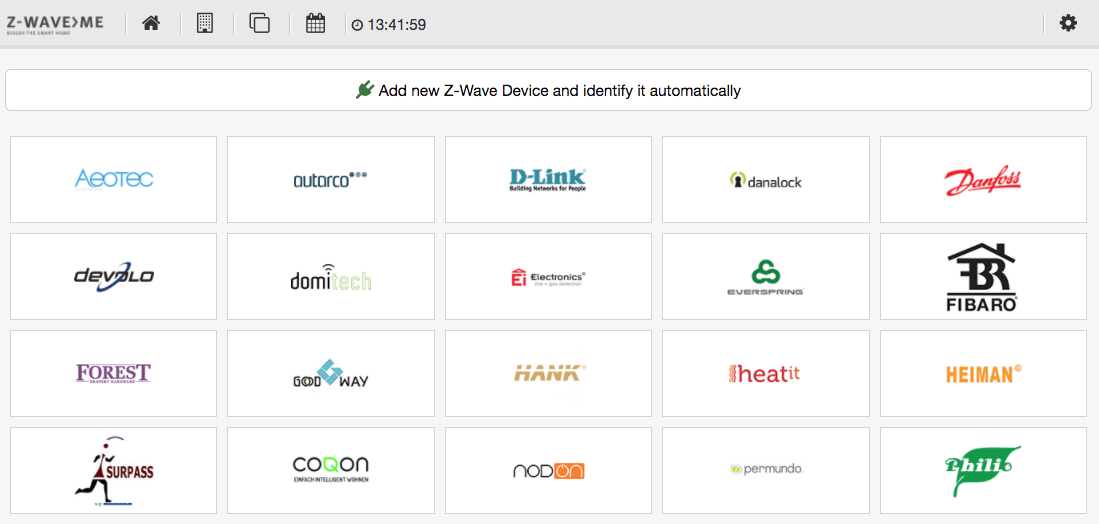
\includegraphics[width=0.9\textwidth]{pngs/cap4/device1.png}
\caption{\zwave Device Vendor Overview}
\label{device1}
\end{center}
\end{figure}

To include a new \zwave device (one of the first steps needed to start a smart home 
system!) please click on the ``+’’ button on the \zwave device part. This will open an 
overview of current \zwave device vendors by name and logo. Figure \ref{device1} 
shows this overview.

Generally, there is no need to know the \zwave brand and product code. All \zwave devices 
are self-describing, and automatically identified products will provide the same functions 
as the devices that were pre-identified. Thus, experienced users will always click on 
the upper button to add a new unidentified \zwave device. The only reason to find a 
specific device from the list is to get some additional information on how to include this 
device. This refers to the button and the button push sequence needed for inclusion.

Since most \zwave devices have one \zwave inclusion button and single or triple click 
will do the inclusion, this information is only needed for some devices with exotic 
inclusion options. Both the buttons to include an unknown device and the right-hand 
side button of an identified button will lead to the same inclusion dialog as 
shown in Figure \ref{device3}.

\begin{figure}
\begin{center}
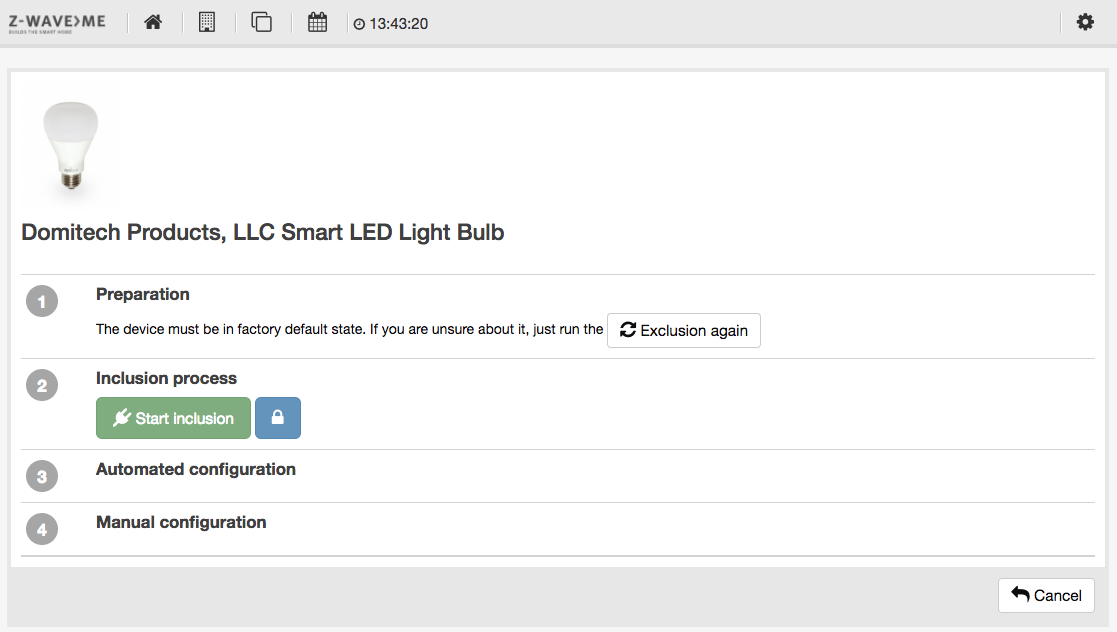
\includegraphics[width=0.9\textwidth]{pngs/cap4/device3.png}
\caption{\zwave Device Inclusion Dialog}
\label{device3}
\end{center}
\end{figure}

\framebox{\textbf{It is recommended to exclude (reset) a device before it gets included}.}


However, 
if you are sure that the device is new and in factory default state, you may skip this 
step. Right next to the inclusion button there is another small button that defines if the 
device will be included with special security functions. By default, the security option 
is enforced. However, some devices in the market may not work as expected using the 
security function. In case there is a connection problem, unsecure inclusion may still work.

Once the inclusion mode has been started, the controller waits for devices to be 
included. Figure \ref{incl1} shows the controller at this moment. The inclusion mode can 
be terminated using the same button. Any new device included will also terminate the process.

\begin{figure}
\begin{center}
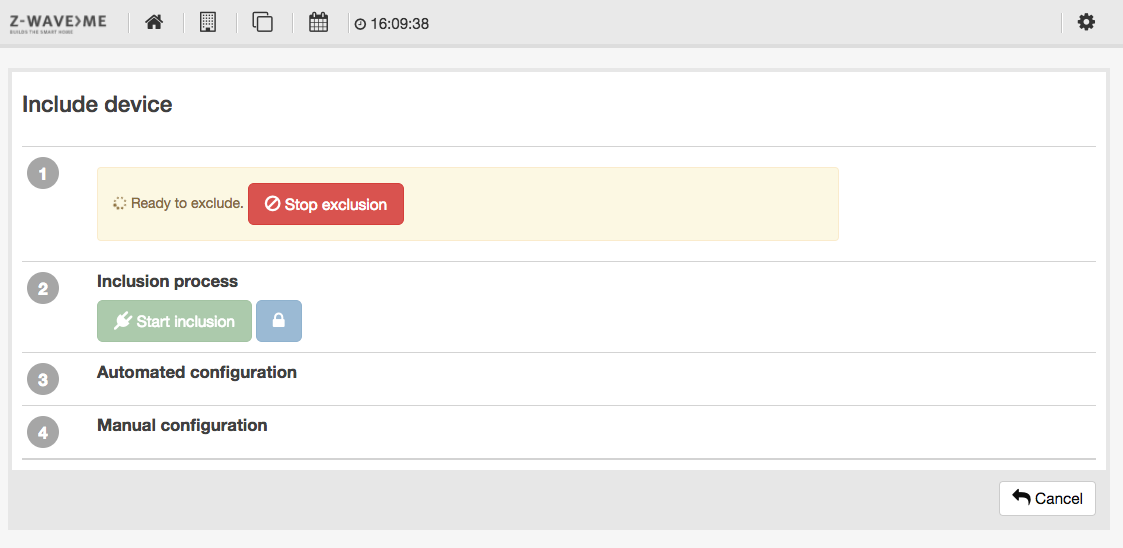
\includegraphics[width=0.9\textwidth]{pngs/cap4/incl1.png}
\caption{\zwave Device Exclusion Dialog}
\label{incl1}
\end{center}
\end{figure}

\begin{figure}
\begin{center}
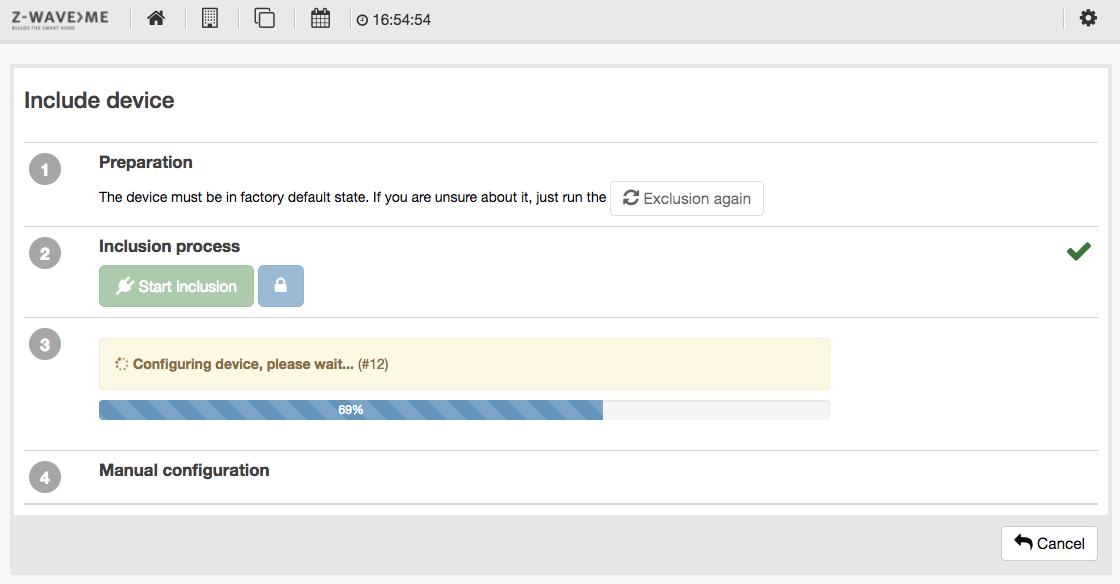
\includegraphics[width=0.9\textwidth]{pngs/cap4/incl2.png}
\caption{\zwave Device Successful Inclusion}
\label{incl2}
\end{center}
\end{figure}

In case the new device requires authorization, this needs to be done 
right after inclusion.
Authorization ensures that the device that appears on the user interface is indeed the 
device in hand. To ensure this the device offers either a QR code to be read or a 
device individual PIN number, both types of information need to be provided to the user 
interface manually.
The controller will then match the information provided by the user with the information 
provided by the device using wireless communication. Only in case they match the device 
can be used.

\begin{figure}
\begin{center}
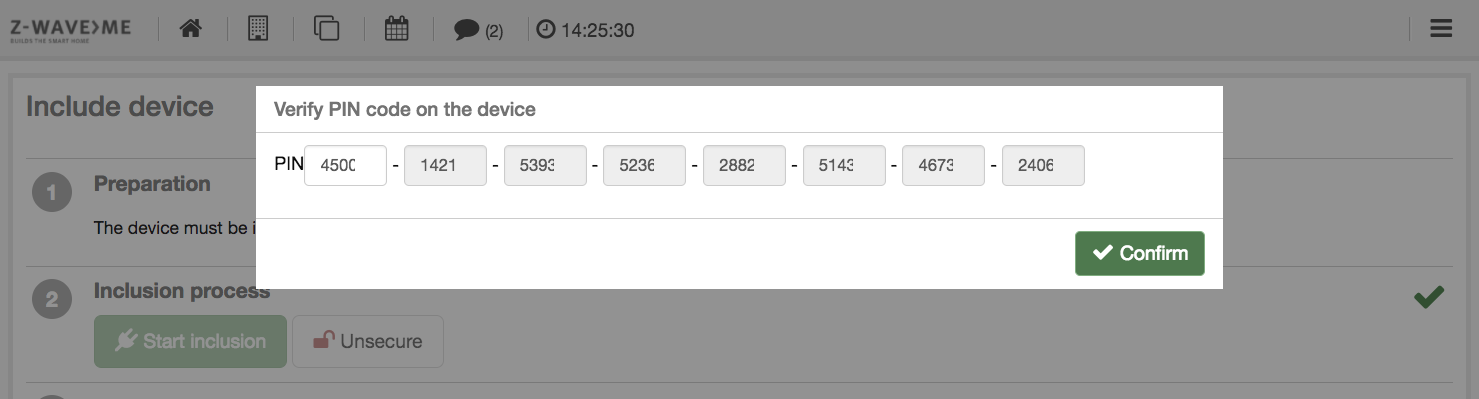
\includegraphics[width=0.9\textwidth]{pngs/cap4/SHUI_S2AUTH.png}
\caption{\zwave Device Authentication}
\label{security2_6}
\end{center}
\end{figure}

Authentication is only required for certain devices. In this case, a 
window like that shown in Figure \ref{security2_6} pops up asking for the authentication 
information. Once given, they are checked. If authentication fails, a warning is 
displayed. It is not possible to just repeat the authentication. The 
device must be excluded and re-included.


Any new device will be interviewed next. In this process, all functions announced by 
the device itself will be verified and certain user interface relevant data will be called 
from the device. A progress bar such as that in Figure \ref{incl2} shows the status.

Once the interview was passed successfully, a dialog offers some initial manual configuration 
functions, as shown in Figure \ref{device3}:

\begin{figure}
\begin{center}
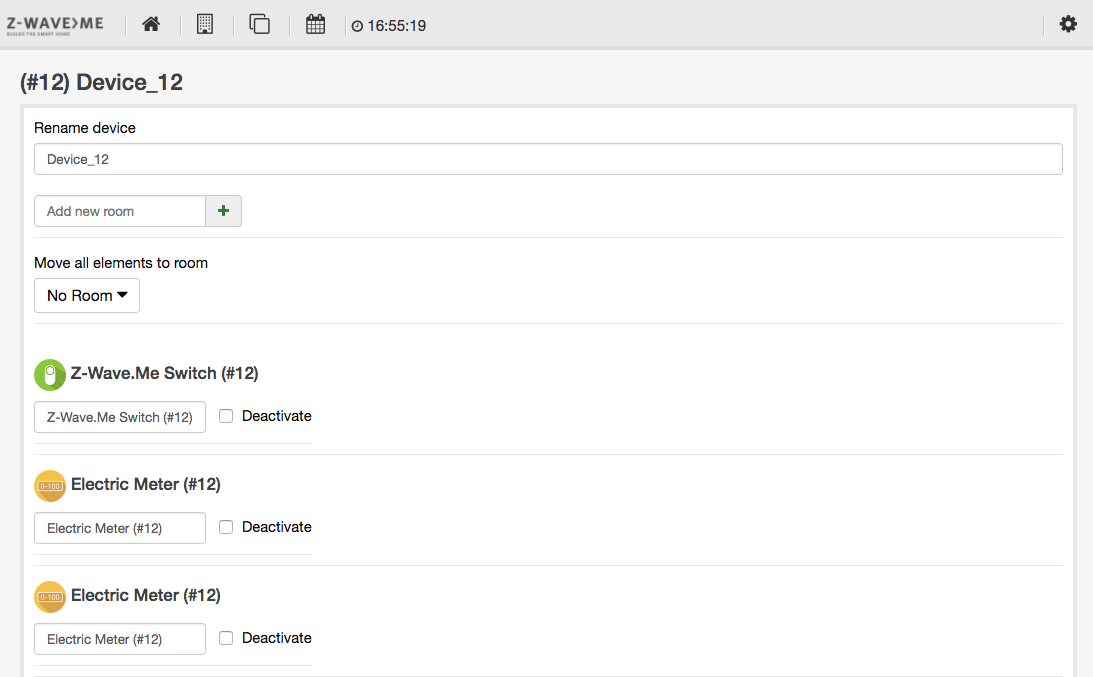
\includegraphics[width=0.9\textwidth]{pngs/cap4/incl3.png}
\caption{\zwave Device manual configuration}
\label{incl3}
\end{center}
\end{figure}

\begin{itemize}
\item Rename the device as such. This device name only refers to the physical device and 
will not be shown in the standard user interface. Use descriptive words 
like ``Popp Smoke on sealing’’ to re-identify the device later.
\item It is possible to move all elements shown below into one single room. If this is not 
done here, it is still possible to move each element on the configuration dialog as 
described in Section \ref{ElementConfiguration}.
\item The list of the elements generated by the new device. Here you can change the name 
that will then appear on the element overview, etc. You can also deactivate the element 
if you don’t see any need to have it.
\item Some physical devices offer further hardware-specific settings such as wakeup interval 
time. If the new device offers such configuration, another button for hardware 
configuration is shown. Please refer to the \zweui 
configuration description in Chapter \ref{Configuration} for more information on how to 
use this dialog. Both dialogs are identical.
\end{itemize}

\begin{figure}
\begin{center}
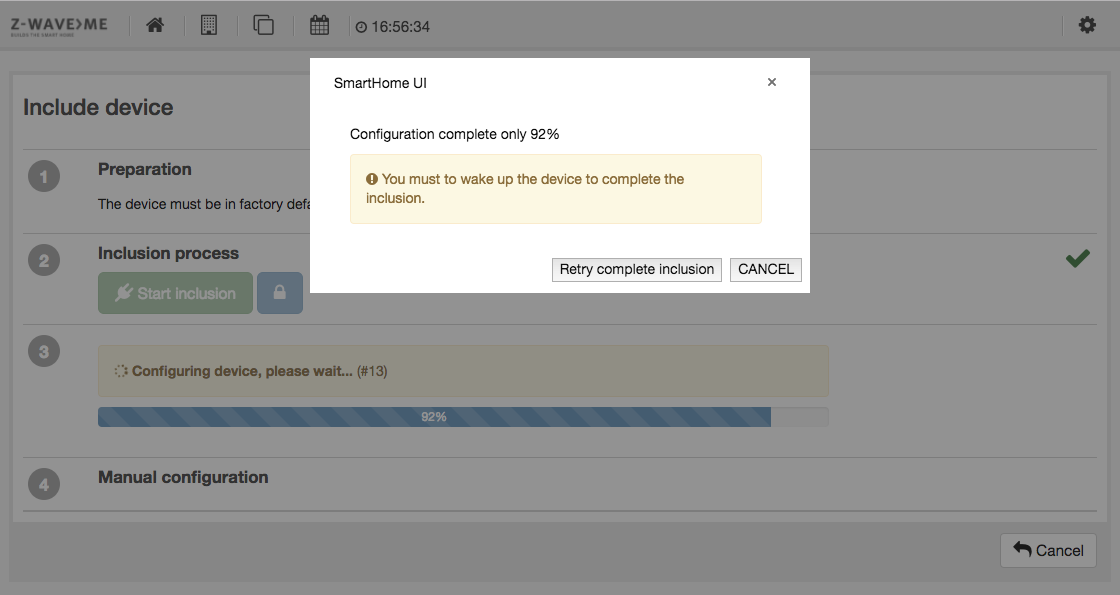
\includegraphics[width=0.9\textwidth]{pngs/cap4/incl4.png}
\caption{\zwave device inclusion failed}
\label{incl4}
\end{center}
\end{figure}

The interview process does not only detect all information from the device; it also tests 
the connectivity of the device. Certain communication may fail. Another good reason for 
such a failure is that a battery-operated device goes into deep sleep mode too fast. 
Figure \ref{incl4} shows the error message in case of failure. In most cases, it’s OK to 
just redo the interview and wake up the device.

If the second attempt at the interview fails, the controllers gives the option to 
accept the result or to redo the entire process. Figure \ref{incl5} shows this dialog box.

\begin{figure}
\begin{center}
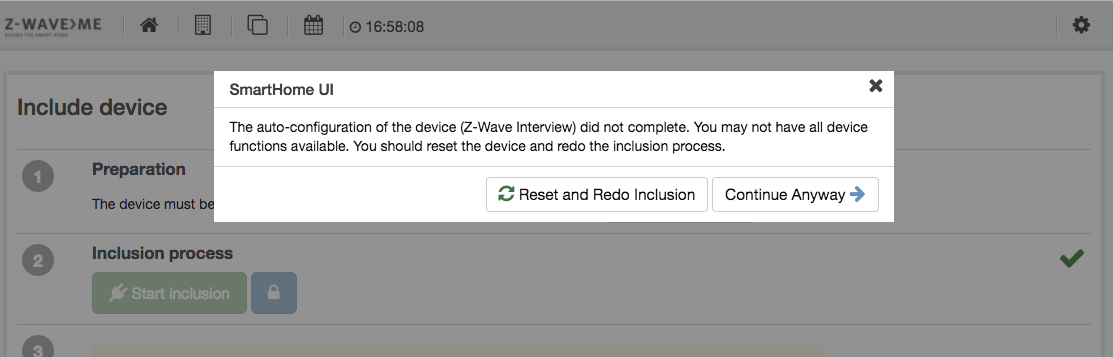
\includegraphics[width=0.9\textwidth]{pngs/cap4/incl5.png}
\caption{\zwave device inclusion repeated}
\label{incl5}
\end{center}
\end{figure}

Once the interview has passed and all configurations are done, the device can be used.

\subsubsection{\zwave Device Management}

The second option for \zwave devices besides adding (including) new devices is the device 
management menu. Clicking on the ``Manage’’ button opens a menu with three tabs:

\begin{itemize}
\item Figure \ref{incl6} shows a list of the physical \zwave devices. The \keystroke{*} button 
will open the very same device management dialog as described during manual post-inclusion 
configuration in Section \ref{inclusion}.
\item Figure \ref{incl7} shows the battery status overview. The list can be ordered by 
the battery charging level.
\item Figure \ref{incl8} shows a list of network status messages. This can be warnings 
for empty battery, devices lost, devices replaced, etc. Clicking on the device name 
lists all the elements created by this physical device.
\end{itemize}


\begin{figure}
\begin{center}
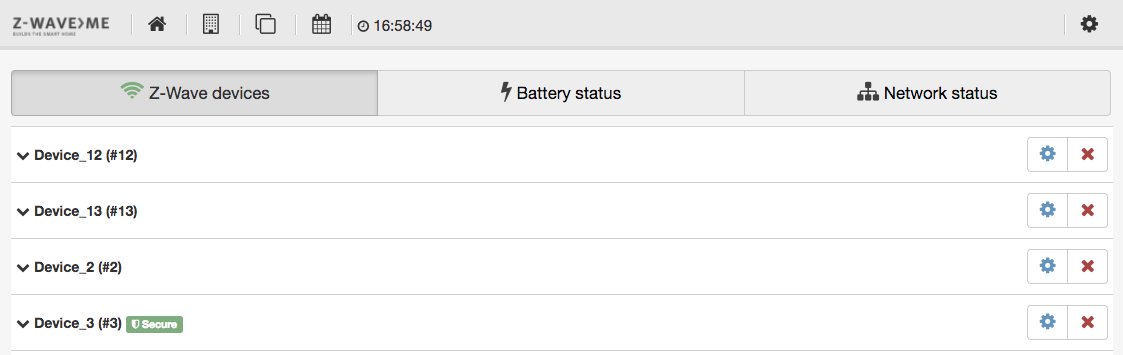
\includegraphics[width=0.9\textwidth]{pngs/cap4/incl6.png}
\caption{\zwave device overview}
\label{incl6}
\end{center}
\end{figure}

\begin{figure}
\begin{center}
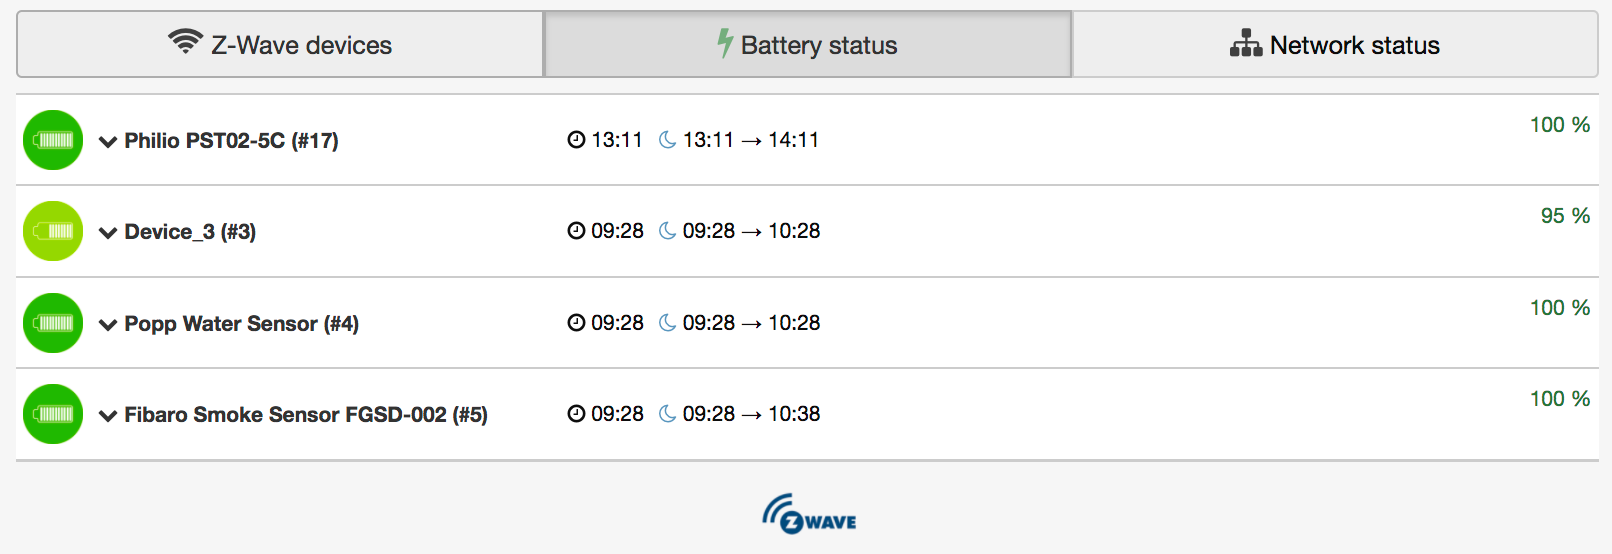
\includegraphics[width=0.9\textwidth]{pngs/cap4/incl7.png}
\caption{\zwave device battery overview}
\label{incl7}
\end{center}
\end{figure}

\begin{figure}
\begin{center}
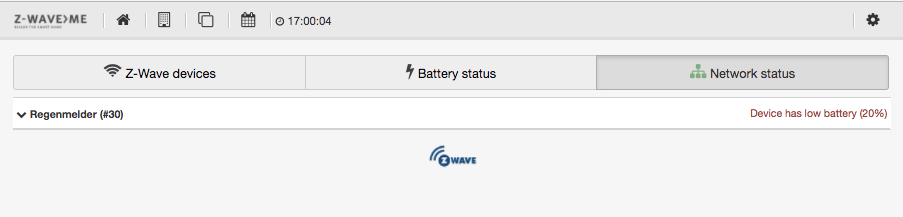
\includegraphics[width=0.9\textwidth]{pngs/cap4/incl8.png}
\caption{\zwave device network status}
\label{incl8}
\end{center}
\end{figure}

\subsection{Customize}
\label{customize}


The customization menu option allows changing the look and feel of your \zway user 
interface. You can add more icons as device-specific icons and you can change the look 
and feel using skins. For more information on skins and how to create them, please refer 
to Chapter \ref{MakeSkins}. This menu here only deals with skins that are already available.

The menu offers four tabs. The tab shown in Figure \ref{shui81} shows the list of skins 
locally available. They can be activated by just clicking on the green activation button.

\begin{figure}
\begin{center}
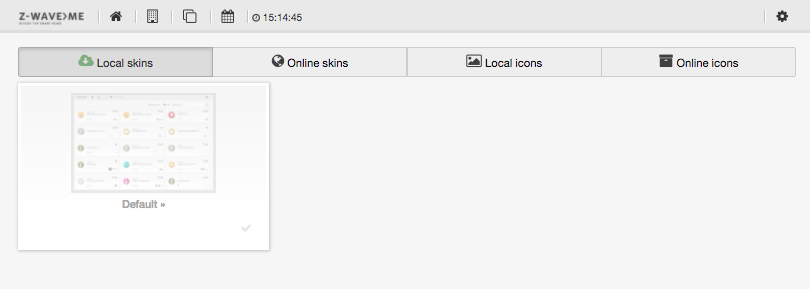
\includegraphics[width=0.9\textwidth]{pngs/cap4/shui81.png}
\caption{Local Skins}
\label{shui81}
\end{center}
\end{figure}

The tab shown in Figure \ref{shui82} offers the list of skins available for download. 
They must be downloaded first before they can be activated and applied.

\begin{figure}
\begin{center}
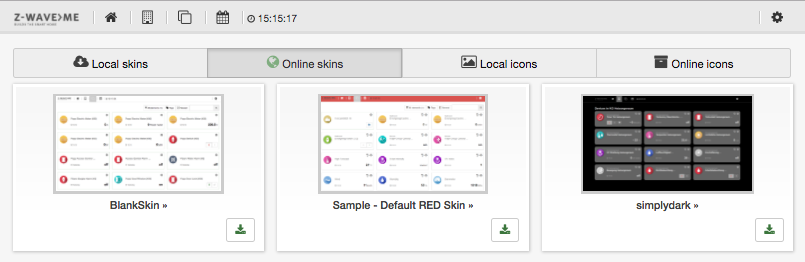
\includegraphics[width=0.9\textwidth]{pngs/cap4/shui82.png}
\caption{Skins on Server}
\label{shui82}
\end{center}
\end{figure}

The tab shown in Figure \ref{shui83} lists the additional icons available on the controller. 
They can be activated per element on the element configuration menu described in 
Chapter \ref{ElementConfiguration}.


\begin{figure}
\begin{center}
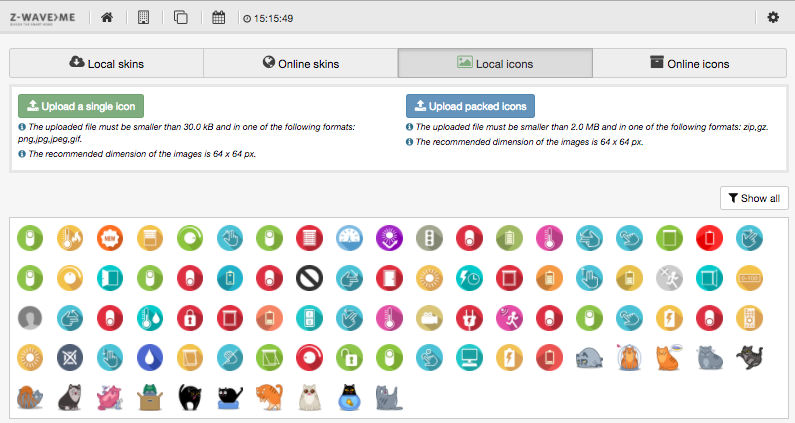
\includegraphics[width=0.9\textwidth]{pngs/cap4/shui83.png}
\caption{Local Icons}
\label{shui83}
\end{center}
\end{figure}

The tab shown in Figure \ref{shui84} offers additional icon sets available on the server. 
They must be downloaded first before they can be activated and applied.

\begin{figure}
\begin{center}
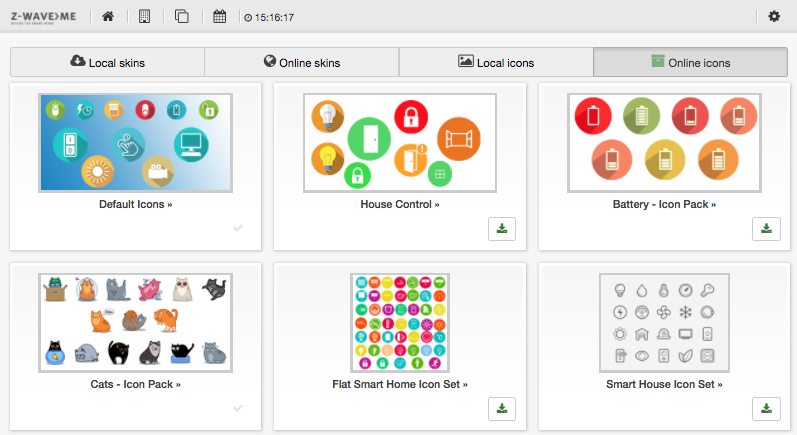
\includegraphics[width=0.9\textwidth]{pngs/cap4/shui84.png}
\caption{Icon-Sets on Server}
\label{shui84}
\end{center}
\end{figure}

\subsection{My Settings}
\label{mysettings}
\index{My Settings}

In this dialog, as shown in Figure \ref{device4}, the local user interface settings for 
the logged in user can be changed.

\begin{itemize}
\item Name: This is the name of the account. Even if this name is changed, the login name is NOT changed.
\item Email: This email is used for certain email notifications, for password recovery and for the recovery of cloud backups.
\item Language: Click on the flags to change the user interface language.
\item UI update rate: This is the refresh rate for the user interface web pages.
\item Expert View: Having the checkbox marked shows some system apps in the overview of 
running apps that are not shown by default. For more information on apps, please refer 
to Chapter \ref{apps}.
\item Events: The two checkboxes allow suppressing certain events. They are then removed 
from the timeline and will not create any out-of-band alert.
\item Hidden events of devices:  This 
is a list of the devices where events are deactivated in the element configuration overview. 
This is the only way to reactivate them if needed. For more information about the element 
configuration, dialog please refer to Chapter \ref{ElementConfiguration}.
\end{itemize}

\begin{figure}
\begin{center}
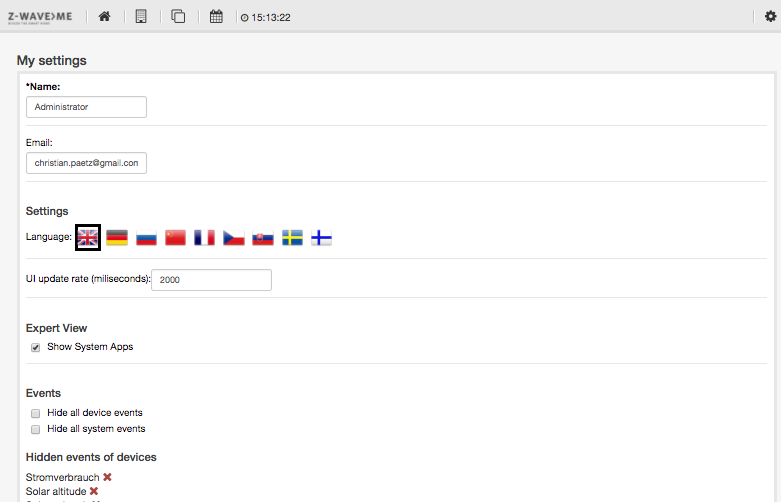
\includegraphics[width=0.9\textwidth]{pngs/cap4/device4.png}
\caption{My Settings Dialog - upper part}
\label{device4}
\end{center}
\end{figure}

Figure \ref{device5} shows the lower part of the \keystroke{Settings} dialog. In \keystroke{My User Account} 
the individual password can be changed.

The section \keystroke{Add mobile device} shows a QR code to simplify the setup. Please refer to 
Section \ref{mobileapps} for more information on how to use this QR code.


\begin{figure}
\begin{center}
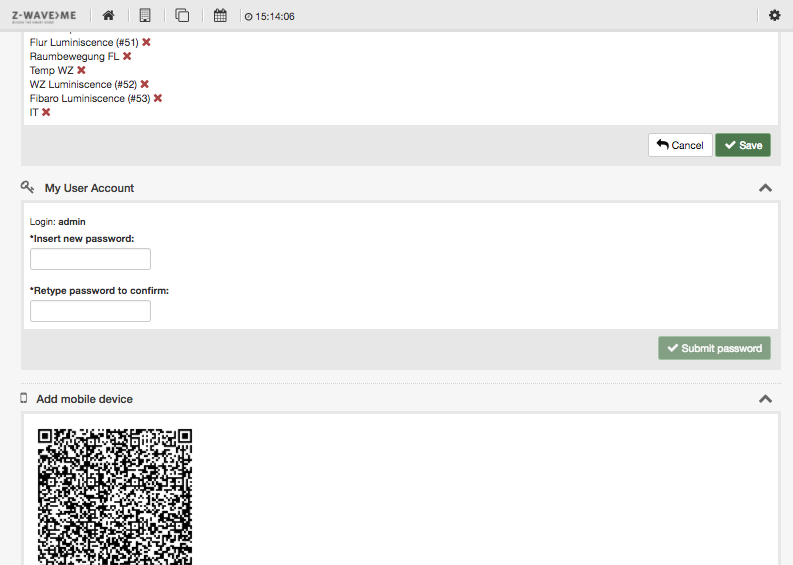
\includegraphics[width=0.9\textwidth]{pngs/cap4/device5.png}
\caption{My Settings Dialog - lower part}
\label{device5}
\end{center}
\end{figure}

\subsection{Management}

The menu item \keystroke{Management} opens a new menu with options to technically manage the platform. 
These management options are available for administrators only. Please refer to Section 
\ref{ManagementInterface} for more information about the management options.

\subsubsection{News}
\label{news}

\begin{figure}
\begin{center}
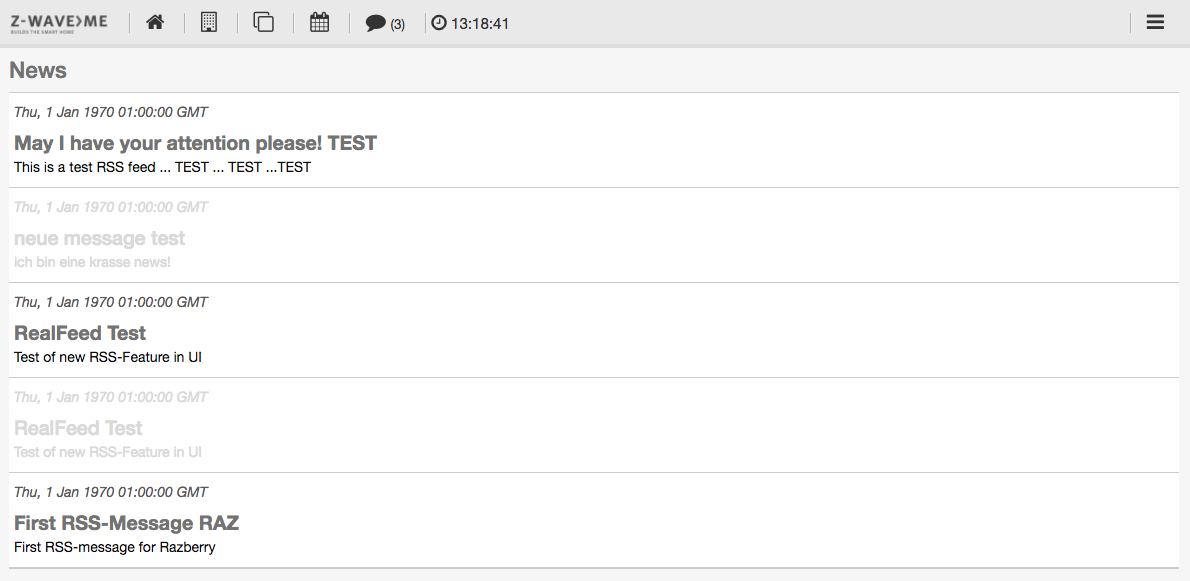
\includegraphics[width=0.9\textwidth]{pngs/cap4/news2.png}
\caption{List of \zway news}
\label{news2}
\end{center}
\end{figure}

As shown in Figure \ref{news2}, this dialog lists all news entries received from the RSS feed.

\subsubsection{Logout}

The logout button cancels the user sessions of the \zwshui. In case of 
a login from find.zwave.me, the user is redirected to the find.zwave.me overview page or 
else to the local login page.

\section {The Management Interface}
\label{ManagementInterface}

Figure \ref{shui91} shows the controller management menu. \textbf{Please note that this 
menu is available for users with administrator privileges} only.

\begin{figure}
\begin{center}
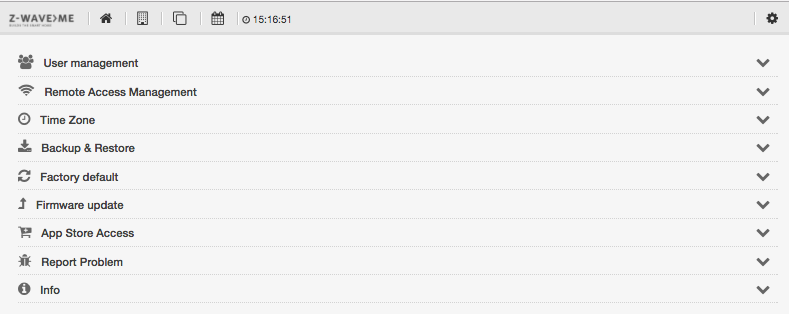
\includegraphics[width=0.9\textwidth]{pngs/cap4/shui91.png}
\caption{Administrator Management Menu}
\label{shui91}
\end{center}
\end{figure}

\subsection{User Management}


Figure \ref{shui71} shows the list of users. It is possible to add more users, change 
their settings, and remove them. Clicking on the setup button opens the user setup dialog. 
It allows managing

\begin{itemize}
\item Name and Email
\item Role types: This defines the access rights of the user account. Admin allows 
accessing the management submenu. Standard users will be role-type ``users.’’ It is 
possible to further restrict a user account to real local access or to make it an 
anonymous user.
\item Language of the user interface
\item Password settings
\end{itemize}

\begin{figure}
\begin{center}
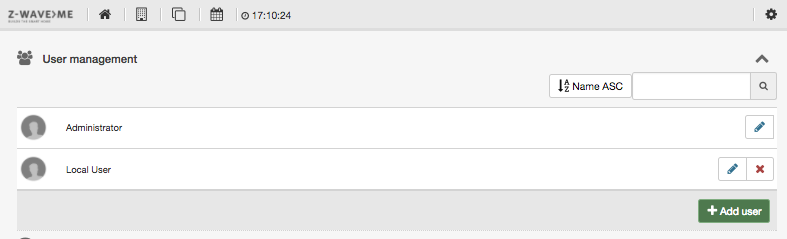
\includegraphics[width=0.9\textwidth]{pngs/cap4/shui71.png}
\caption{User Management}
\label{shui71}
\end{center}
\end{figure}

\subsection{Remote Access Management}
\index{Remote Access}


The dialog shown in Figure \ref{shui72} allows managing the remote access functions of 
the controller. By default, the remote access function is activated. This enables accessing 
the controller from any end device in the Internet, e.g. a mobile phone. Please refer 
to Chapter \ref{remoteaccess} for information on how this remote access is implemented 
and what security implications this function has.

The remote support function is deactivated by default. This function allows support 
staff with access rights to the remote access server to remotely access your controller 
using remote shell (ssh). For complicated support issues, the support staff may ask 
to activate this function. Please make sure to deactivate it after the session. The 
remote ssh is only accessible to support staff with support infrastructure rights.
 Nevertheless, there is no good reason to keep a port open if not needed.

\begin{figure}
\begin{center}
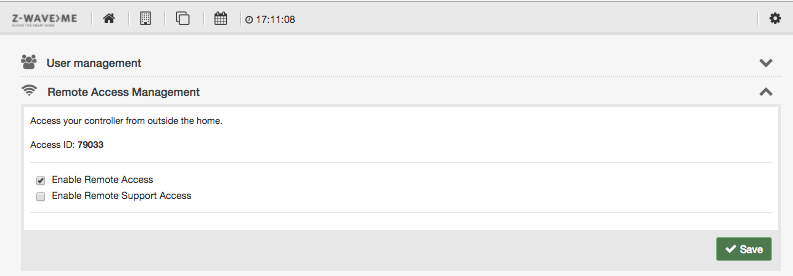
\includegraphics[width=0.9\textwidth]{pngs/cap4/shui72.png}
\caption{Remote Access Management}
\label{shui72}
\end{center}
\end{figure}

\subsection{Time Zone}
\index{Time Zone}

The dialog shown in Figure \ref{shui73} allows managing the time zone of the controller. 
This ensures that all time stamps and the time clock on the top menu bar refer correctly 
to the local time at the location of the server. Please note that the time remains 
unchanged if you access the device from a browser from a different time zone.

\begin{figure}
\begin{center}
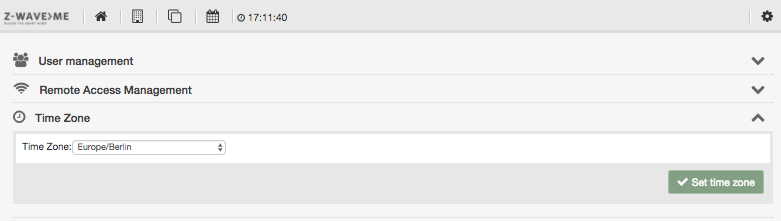
\includegraphics[width=0.9\textwidth]{pngs/cap4/shui73.png}
\caption{Time Zone Management}
\label{shui73}
\end{center}
\end{figure}

\subsection{Backup \& Restore}
\index{Backup \& Restore}

Backup and restore can be done in two different ways:

\begin{itemize}
\item Time driven and automated into the \zway cloud service.
\item Manually triggered into filesystem of PC running the web browser.
\end{itemize}

The first block of the \keystroke{Backup \& Restore} dialog controls the cloud backup, which 
can be activated or deactivated, as shown in Figure \ref{shui74}. When activated, the 
controller will automatically generate a backup file and send it to the cloud server 
using SSL encryption.

The files are stored on a server managed by \zwaveme. This is a convenient way to keep 
and update a backup file---and its free of charge. However, if you don’t trust this 
server or the company, just don’t use cloud backup!

The cloud backup interface allows defining the backup interval and the notification in 
terms of failed or successful backup performed.

\begin{figure}
\begin{center}
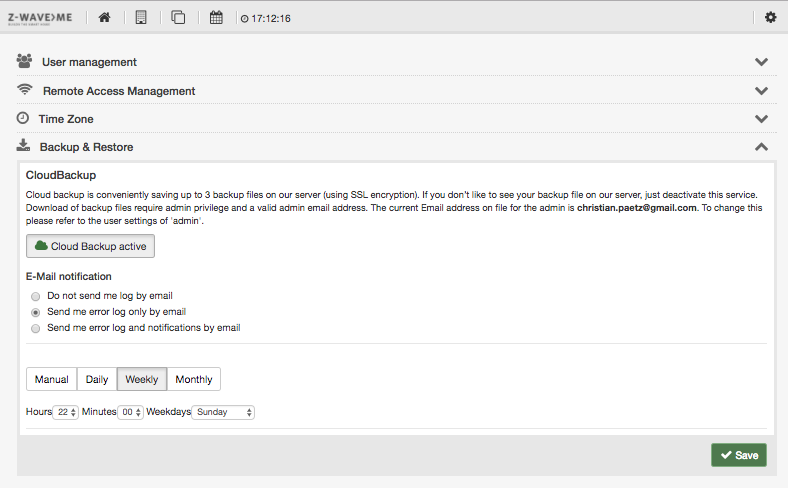
\includegraphics[width=0.9\textwidth]{pngs/cap4/shui74.png}
\caption{Automated Backup into Cloud}
\label{shui74}
\end{center}
\end{figure}

The local backup option, as shown in Figure \ref{shui75}, will generate a local backup 
file that needs to be stored on the local hard drive of the PC running the web browser. 
The file is identical to the file stored in the cloud. From the technical side, this is 
a ZIP file that can even be decompressed and audited. It will comprise XML and JSON files 
and images that were uploaded before.

\begin{figure}
\begin{center}
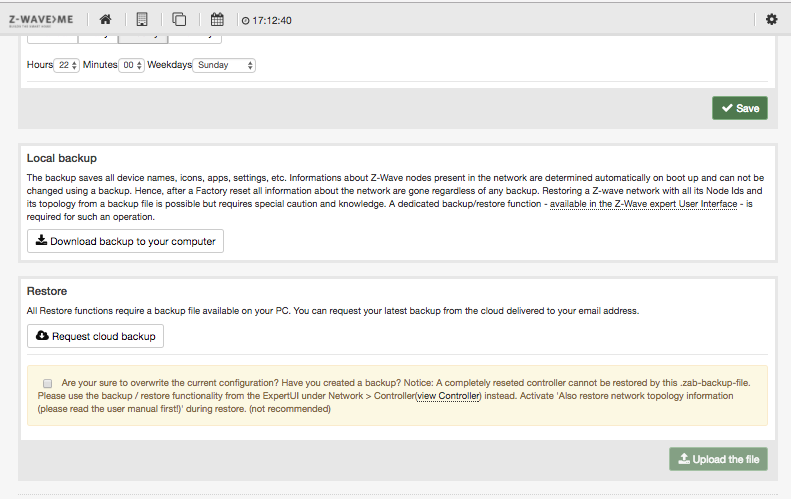
\includegraphics[width=0.9\textwidth]{pngs/cap4/shui75.png}
\caption{Local Back and Restore}
\label{shui75}
\end{center}
\end{figure}

If the cloud backup option was chosen, the backup file needs to be downloaded to the 
local PC before being applied as a restore file. Clicking on the button ``Request Cloud Backup’’ 
will cause the server to generate a temporarily valid token which is sent by mail to the 
mail address defined for the admin account. This email will contain an explanation of the 
process and a unique link to an online list of backup files available. Just download the file of choice.

The real restore function always requires a file uploaded from the local file system. A 
checkbox ensures that the user understands the consequences of applying a restore file.

Please note that the backup and restore function will only handle files on the controller, 
and not the \zwave network topology stored in the \zwave transceiver chip.

To overwrite this content, please refer to the \zweui, as 
described in Chapter \ref{BackupandRestore}.


\subsection{Factory default}
\index{Reset}

This function resets all functions of the controller. All uploaded images will be deleted 
and all given names and settings will be removed. The included \zwave devices will NOT be 
removed. For removing them from the controller, please refer to the basic \zwave 
literature, e.g. the book ``Z-Wave Essentials’’ as mentioned in Chapter \ref{cap1}.


\subsection{Firmware Update}
\index{Firmware Update}

The firmware update menu as shown in figure \ref{shui76} refers to two different processes:

\begin{itemize}
\item \keystroke{Update device database}: This button can be triggered to update the \zwave device 
database used for the inclusion process described in Chapter \ref{inclusion}. This 
update is not critical and new firmware updates will update this device database 
anyway. However, for debugging purposes, it is sometimes beneficial to force a database update.
\item \keystroke{Firmware Update}: This option will update the whole firmware including the dialog 
offering this update.
\end{itemize}

\begin{figure}
\begin{center}
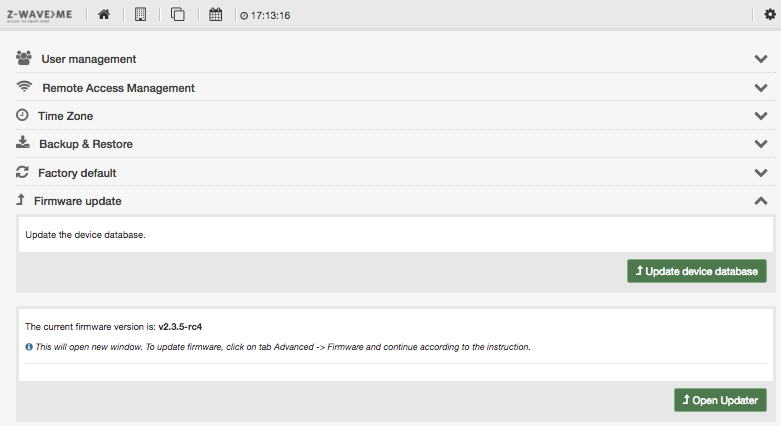
\includegraphics[width=0.9\textwidth]{pngs/cap4/shui76.png}
\caption{Firmware Update Options}
\label{shui76}
\end{center}
\end{figure}

Updating the firmware is a quite complex process. In the normal operation mode, all 
communication between user interface and controller backend is handled using IP Port 8083. 
However, there are good reasons not to use this port for the management of the firmware update:

\begin{itemize}
\item The update script will overwrite the same software that informs about the update as such.
\item In case the update fails, or the update firmware is damaged and not working correctly, 
there is no way to turn the update back since the dialog doing so (on port 8083) will not 
be available anymore.
\end{itemize}

This is why hitting the button \keystroke{Open Updater} will open a new user interface embedded 
into the current interface. Figure \ref{shui77} shows this new black-background user 
interface dedicated to the firmware update function. This user interface is served from 
another webserver temporarily active on IP port 8084. Hence, it would be possible to 
directly access this user interface using the


\murl{http://MYIP:8084}.


This user interface will remain active for about 10 minutes. This is enough time to perform
 the firmware update and revert it in case of problems. After the 10 minutes, the service on 
 8084 is deactivated automatically.

\begin{figure}
\begin{center}
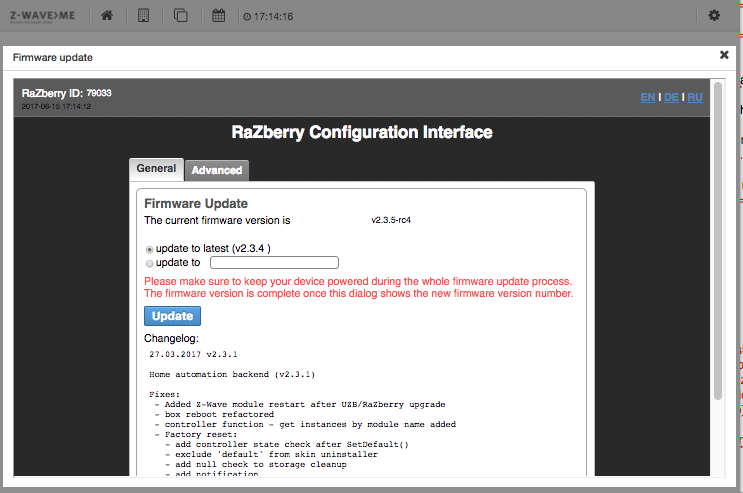
\includegraphics[width=0.9\textwidth]{pngs/cap4/shui77.png}
\caption{Firmware Update Dialog}
\label{shui77}
\end{center}
\end{figure}

The firmware update dialog shows the current firmware and offers update to the most recently 
released firmware version. For debugging or trouble shooting purposes, it is possible to load 
a specific firmware version. A change log shows the changes of all the official firmware 
release versions.

\subsection{App Store Access}

The app store allows downloading new apps provided either by \zwaveme or other independent 
developers. Some of these developers may want to limit the use of their apps to a 
certain group of people, either because this is related to their business model, or 
because the apps are beta stage or for trial only.

The token concept is a simple and efficient method to limit access. Apps that are uploaded 
to the app server (For more information on how to create and upload apps, please refer 
to Chapter \ref{apps}) can be marked with one or more tags. These tags are simple strings 
and the developer can choose whatever token he wants. He can also have more than one tag 
for different purposes.

In order to access apps that are tagged, the various tags need to be added to the 
controller using the form shown in Figure \ref{shui78}. Tags can be added and removed. 
Once a tag is added, all the apps with this tag will be shown in the app store, as 
described in Section \ref{appssetup}.


\begin{figure}
\begin{center}
\includegraphics[width=0.9\textwidth]{pngs/cap4/shui78.png}
\caption{App Store Access}
\label{shui78}
\end{center}
\end{figure}

\subsection{Report Problem}

The menu item, as shown in Figure \ref{shui79}, demonstrates a quick and simple way to 
report bugs and problems related to this User Interface. Providing an email is optional, 
but please be aware that the form will transmit some meta data such as version number of 
the User Interfaces or version number of the firmware. If you don’t like to share such 
information, please use your personal email. Also, please don’t expect an individual 
answer to the bug reports. This is not a support tool.


\begin{figure}
\begin{center}
\includegraphics[width=0.9\textwidth]{pngs/cap4/shui79.png}
\caption{Problem Reporting Form}
\label{shui79}
\end{center}
\end{figure}

\subsection{Info}

The info menu item provides some version information for the user interface and the 
backend. This information is usually needed for support and troubleshooting purposes only.
